\documentclass[12pt]{amsart}
%prepared in AMSLaTeX, under LaTeX2e
\addtolength{\oddsidemargin}{-.65in} 
\addtolength{\evensidemargin}{-.65in}
\addtolength{\topmargin}{-.55in}
\addtolength{\textwidth}{1.3in}
\addtolength{\textheight}{.8in}

\renewcommand{\baselinestretch}{1.05}

\usepackage{verbatim} % for "comment" environment

\usepackage{palatino}

\newtheorem*{thm}{Theorem}
\newtheorem*{defn}{Definition}
\newtheorem*{example}{Example}
\newtheorem*{problem}{Problem}
\newtheorem*{remark}{Remark}

\usepackage{fancyvrb,xspace,dsfont}

\usepackage[final]{graphicx}

% macros
\usepackage{amssymb}

\usepackage{hyperref}
\hypersetup{pdfauthor={Ed Bueler},
            pdfcreator={pdflatex},
            colorlinks=true,
            citecolor=blue,
            linkcolor=red,
            urlcolor=blue,
            }

\newcommand{\br}{\mathbf{r}}
\newcommand{\bv}{\mathbf{v}}
\newcommand{\bx}{\mathbf{x}}
\newcommand{\by}{\mathbf{y}}

\newcommand{\cB}{\mathcal{B}}
\newcommand{\cD}{\mathcal{D}}
\newcommand{\cF}{\mathcal{F}}
\newcommand{\cH}{\mathcal{H}}
\newcommand{\cL}{\mathcal{L}}
\newcommand{\cV}{\mathcal{V}}
\newcommand{\cW}{\mathcal{W}}

\newcommand{\CC}{\mathbb{C}}
\newcommand{\NN}{\mathbb{N}}
\newcommand{\RR}{\mathbb{R}}
\newcommand{\ZZ}{\mathbb{Z}}

\renewcommand{\Im}{\mathrm{Im}}
\renewcommand{\Re}{\mathrm{Re}}

\newcommand{\eps}{\epsilon}
\newcommand{\grad}{\nabla}
\newcommand{\lam}{\lambda}
\newcommand{\lap}{\triangle}

\newcommand{\ip}[2]{\ensuremath{\left<#1,#2\right>}}

\newcommand{\image}{\operatorname{im}}
\newcommand{\onull}{\operatorname{null}}
\newcommand{\rank}{\operatorname{rank}}
\newcommand{\range}{\operatorname{range}}
\newcommand{\trace}{\operatorname{tr}}
\newcommand{\Span}{\operatorname{span}}

\newcommand{\prob}[1]{\bigskip\noindent\textbf{#1.}\quad }

\newcommand{\pts}[1]{(\emph{#1 pts}) }
\newcommand{\epart}[1]{\medskip\noindent\textbf{(#1)}\quad }
\newcommand{\ppart}[1]{\,\textbf{(#1)}\quad }

\newcommand{\ds}{\displaystyle}

\newcommand{\nex}{\medskip\noindent}


\begin{document}
\scriptsize \noindent Math 617 Functional Analysis (Bueler) \hfill \emph{version 1; assigned 22 April 2024}
\normalsize\medskip

\Large\centerline{\textbf{Assignment 8}}
\large
\medskip

\centerline{\textbf{Due at 12:00pm NOON on Thursday 2 May 2024}}
\medskip
\normalsize

\thispagestyle{empty}

\bigskip
\noindent This Assignment is based on sections 4.1, XX of our textbook, Borthwick (2020)~\emph{Spectral Theory: Basic Concepts and Applications}, Springer.

\medskip
\noindent \textsc{Please do the following exercises.}
\smallskip

\renewcommand{\SS}{\mathbb{S}}


% Exer 4.4, but made specific to \ell^2
\prob{P38}  \emph{The basic facts in Lemma 4.3 and Theorem 4.4 are important in this problem.  You have already shown (on the Midterm Quiz!) that $R$ has no eigenvalues.}

\medskip\noindent Let $R$ be the right shift on $\cH=\ell^2$, a bounded operator:
	$$R (a_1,a_2,a_3,\dots) = (0,a_1,a_2,\dots).$$

\epart{a}  Show that $L=R^*$ is the left shift, and that $\|R\|=\|L\|=1$.

\epart{b}  Let $\lambda\in\CC$ such that $|\lambda|<1$.  By constructing an eigenvector, show that $\lambda$ is an eigenvalue of $L$.  (\emph{This requires the eigenvector be in $\cH$!})

\epart{c}  Find $\sigma(L)$ and $\sigma(R)$.


% Exer 4.6
\prob{P39}  \emph{By Theorem 4.15, your only job is to show that negative real numbers are in the resolvent set.  One route uses Theorem 3.18, and another (overkill?) uses the spectral theorem.}

\medskip\noindent Prove that the spectrum of a positive self-adjoint operator $A$ satisfies $\sigma(A) \subset [0,\infty)$.


% Exer 4.5
\prob{P40}  \emph{This can be shown using only the geometric series (4.16) and (4.28).  Of course, your job is to show that any $z\in\CC\setminus \SS$ is in the resolvent set.}

\medskip\noindent Let $U$ be a unitary operator on $\cH$.  Show that $\sigma(U) \subset \SS = \{z\in\CC\,:\,|z|=1\}$.


\prob{P41}  Suppose $A$ is a self-adjoint operator on $\cH$.  We apply the (Borel) functional calculus Theorem 5.9.

\epart{a}  Suppose that $0\in\rho(A)$.  Let $f(x)=1$, the constant function.  Show that the functional calculus yields $f(A)=I$.

\epart{b}  If $\rho(A)$ is nonempty and $z\in\rho(A)$, show that
	$$\|(A-z)^{-1}\| = \frac{1}{\operatorname{dist}(z,\sigma(A))}.$$
(\emph{Hint. Construct $f\in\cB_b(\RR)$ to do the job, and use part (b) of Theorem 5.9.})

\epart{c}  Suppose $t\in\RR$ and let $f_t(x) = e^{itx}$ and apply the functional calculus to define $U(t) = f_t(A) = e^{itA}$.  Show that: $U(t)$ is unitary, $U(0) = I$, and $U(t+s) = U(t) U(s)$.  (\emph{In summary, each self-adjoint operator $A$ generates a (commutative) unitary group.})

% Exer 5.5
\prob{P42}  \emph{This is an explanation for why any quantum Hamiltonian operator, which is a self-adjoint operator, generates a unitary time-evolution which preserves total probability.}

\medskip\noindent Suppose $A$ is a self-adjoint operator on $\cH$.  Let $U(t) = e^{itA}$ as in \textbf{P41}.  Show that for $v\in\cD(A)$,
	$$\frac{d}{dt}\Big|_{t=0} (U(t)v) = \lim_{t\to 0} \frac{U(t)v-v}{t} = i A v.$$


\prob{43}  \emph{xx}

The potential $V(x)$ is shown in the figure.

\begin{center}
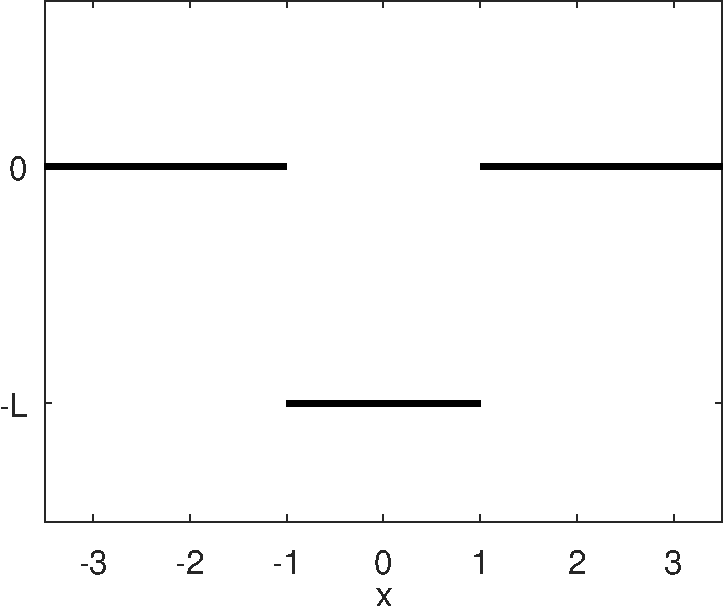
\includegraphics[width=0.4\textwidth]{figs/squarepot.pdf}
\end{center}


\end{document}
